\documentclass[11pt,a4paper]{article}

\usepackage[T1]{fontenc}
\usepackage[utf8]{inputenc}
\usepackage[brazil]{babel}
\usepackage{lmodern}
\usepackage{amsmath,amssymb}
\usepackage{geometry}
\usepackage{booktabs}
\usepackage{listings}
\usepackage{xcolor}
\usepackage{hyperref}
\usepackage{enumitem}
\usepackage{microtype}
\usepackage{titlesec}
\usepackage{float}
\usepackage{graphicx}

\geometry{margin=2cm}
\titlespacing*{\section}{0pt}{2.0ex plus .4ex minus .2ex}{1.0ex}
\titlespacing*{\subsection}{0pt}{1.5ex plus .3ex minus .2ex}{0.7ex}
\hypersetup{colorlinks=true,linkcolor=black,urlcolor=blue,citecolor=black}
\setlist{nosep}
\setlength{\emergencystretch}{2em}
\lstset{
  basicstyle=\ttfamily\small,
  columns=fullflexible,
  keepspaces=true,
  frame=single,
  breaklines=true,
  showstringspaces=false
}

\graphicspath{{../img/}}

\title{NERD - BD -- Etapa 3\\\large JOIN e execução de consultas no modelo materializado: Nested Loop Join, Hash Join e GROUP BY}
\author{Rafael Lima Dias\\Projeto de extensão NERD - BD (Banco de Dados)}
\date{Novembro de 2026}

\begin{document}
\maketitle

\begin{abstract}
Este relatório descreve a etapa 3 do motor de consultas didático do Grupo A, escrito em C11 e baseado no modelo de execução materializado. A etapa acrescenta o suporte a duas tabelas (\texttt{funcionarios} e \texttt{departamentos}), o Nested Loop Join, o Hash Join com fases de BUILD e PROBE explícitas, o GROUP BY por hash e a instrumentação de cada operador. A consulta completa do enunciado foi medida com os dois algoritmos de JOIN, variando a cardinalidade (de 10 mil a 10 milhões de funcionários), a seletividade do filtro (1, 10, 50 e 90\%) e o tamanho da relação de BUILD (de 100 a 100 mil departamentos), com 5 repetições por configuração e mediana. Com 1 milhão de funcionários, a consulta levou 254,5\,ms com Hash Join e 1\,821,7\,ms com Nested Loop; com 10 milhões, 2,7\,s e 19,9\,s. A validação com Valgrind terminou sem vazamentos e sem erros. O relatório traz ainda a arquitetura, as decisões de implementação, o gerenciamento de memória, as dificuldades, as limitações, as otimizações possíveis, o material de extensão e a resposta à questão da etapa.
\end{abstract}

\section{Introdução}
Na etapa 2, o motor executava o pipeline SCAN $\rightarrow$ FILTER $\rightarrow$ PROJECT $\rightarrow$ AGGREGATE sobre uma única tabela. A etapa 3 introduz uma segunda tabela e o operador de JOIN, que é o ponto em que o algoritmo escolhido mais pesa no custo da consulta \cite{graefe,garcia}. No modelo materializado, cada operador consome as entradas inteiras e produz uma tabela completa e independente antes que o operador seguinte comece. A consulta de referência é
\par\medskip\noindent\begin{minipage}{\linewidth}
\begin{lstlisting}[language=SQL]
SELECT d.nome, AVG(f.salario)
FROM funcionarios f
JOIN departamentos d ON f.departamento_id = d.id
WHERE f.salario > 5000
GROUP BY d.nome;
\end{lstlisting}
\end{minipage}\par\medskip
\noindent e é executada pelo plano
\par\medskip\noindent\begin{minipage}{\linewidth}
\begin{lstlisting}[columns=fixed,basicstyle=\ttfamily\footnotesize]
SCAN funcionarios  -> FILTER salary > 5000 --+
                                             +--> JOIN f.department_id = d.id
SCAN departamentos --------------------------+
                                                  |
                                                  v
                                      PROJECT d.name, f.salary
                                                  |
                                                  v
                                      GROUP BY d.name / AVG(f.salary)
\end{lstlisting}
\end{minipage}\par\medskip
O código segue o padrão do repositório, com nomes em inglês: \texttt{departamento\_id}, \texttt{salario}, \texttt{idade}, \texttt{nome} e \texttt{regiao} se chamam \texttt{department\_id}, \texttt{salary}, \texttt{age}, \texttt{name} e \texttt{region}. Os CSV são lidos pela ordem das colunas do esquema.

\textbf{Escopo.} No repositório, cada modelo de execução é de um grupo: Grupo A (Materialização), Grupo B (Pipeline) e Grupo C (Vetorizado). Este trabalho implementa e mede o modelo materializado. As comparações entre modelos (seção 9 do enunciado) e o teste de tamanho de batch (seção 8.4, a cargo do modelo vetorizado) dependem das implementações dos outros grupos e não foram medidas aqui. Quando o texto trata de pipeline ou vetorizado, trata-se de análise do comportamento esperado, e isso é dito explicitamente.

A Tabela~\ref{tab:entregas} relaciona as entregas da seção 11 do enunciado com as partes deste relatório.

\begin{table}[H]
\centering
\small
\begin{tabular}{@{}p{5.0cm}p{11.4cm}@{}}
\toprule
Item do enunciado & Onde está \\
\midrule
11.1 Código & \texttt{src/join.c}, \texttt{src/group\_by.c}, \texttt{src/table.c}, \texttt{src/main.c}, \texttt{include/}, \texttt{tests/}; Seções~\ref{sec:arquitetura} a \ref{sec:testes} \\
11.2 Experimentos & Seção~\ref{sec:experimentos}; dados brutos em \texttt{results/raw/}, gráficos em \texttt{docs/img/} \\
11.3 Documentação técnica & Seções~\ref{sec:arquitetura} a \ref{sec:memoria} e \ref{sec:dificuldades} a \ref{sec:otimizacoes} \\
11.4 Material de extensão & Seção~\ref{sec:extensao} \\
Questão da seção 10 & Seção~\ref{sec:questao} \\
\bottomrule
\end{tabular}
\caption{Entregas da etapa 3.}
\label{tab:entregas}
\end{table}

\section{Arquitetura}\label{sec:arquitetura}

\subsection{Módulos}
A Tabela~\ref{tab:modulos} resume a organização do código nesta etapa.

\begin{table}[H]
\centering
\small
\begin{tabular}{@{}p{5.0cm}p{11.4cm}@{}}
\toprule
Arquivo & Responsabilidade \\
\midrule
\texttt{include/table.h}, \texttt{src/table.c} & \texttt{Schema}, \texttt{Value}, \texttt{Row} (tupla de montagem), \texttt{Table} compacta, leitura de CSV tipada, \texttt{value\_equals} e \texttt{value\_hash} \\
\texttt{include/materialized.h} & API dos operadores, \texttt{QueryMetrics} e \texttt{JoinMetrics} \\
\texttt{src/scan.c} & SCAN, com reserva da capacidade exata \\
\texttt{src/materialized.c} & FILTER e PROJECT \\
\texttt{src/aggregate.c} & AGGREGATE sem agrupamento \\
\texttt{src/join.c} & Nested Loop Join, Hash Join (BUILD e PROBE) e impressão das métricas \\
\texttt{src/group\_by.c} & GROUP BY com índice hash de grupos \\
\texttt{src/main.c} & \texttt{miniquery}: consulta completa com os dois JOINs; datasets opcionais pela linha de comando \\
\texttt{bench/benchmark.c} & \texttt{miniquery\_bench}: consulta instrumentada, uma linha CSV por repetição \\
\texttt{bench/generate\_data.py} & Gerador determinístico de \texttt{funcionarios} e \texttt{departamentos} \\
\texttt{bench/run\_experiments.py} & Gera os datasets, roda os experimentos e grava \texttt{results/raw/} \\
\texttt{bench/summarize.py} & Medianas, tabelas (\texttt{results/tabelas.md}) e gráficos (\texttt{docs/img/}) \\
\texttt{tests/test\_materialized.c} & Testes das etapas 2 e 3 \\
\texttt{Makefile} & Alvos \texttt{all}, \texttt{test}, \texttt{sanitize}, \texttt{valgrind}, \texttt{bench}, \texttt{experiments}, \texttt{clean} \\
\bottomrule
\end{tabular}
\caption{Módulos da etapa 3.}
\label{tab:modulos}
\end{table}

\subsection{Fluxograma}
A Figura~\ref{fig:fluxo} mostra o fluxo da consulta completa, com os dois SCANs, o FILTER, o JOIN (com o BUILD e o PROBE do Hash Join), o PROJECT, o GROUP BY e a ordem de liberação das tabelas.

\begin{figure}[p]
\centering
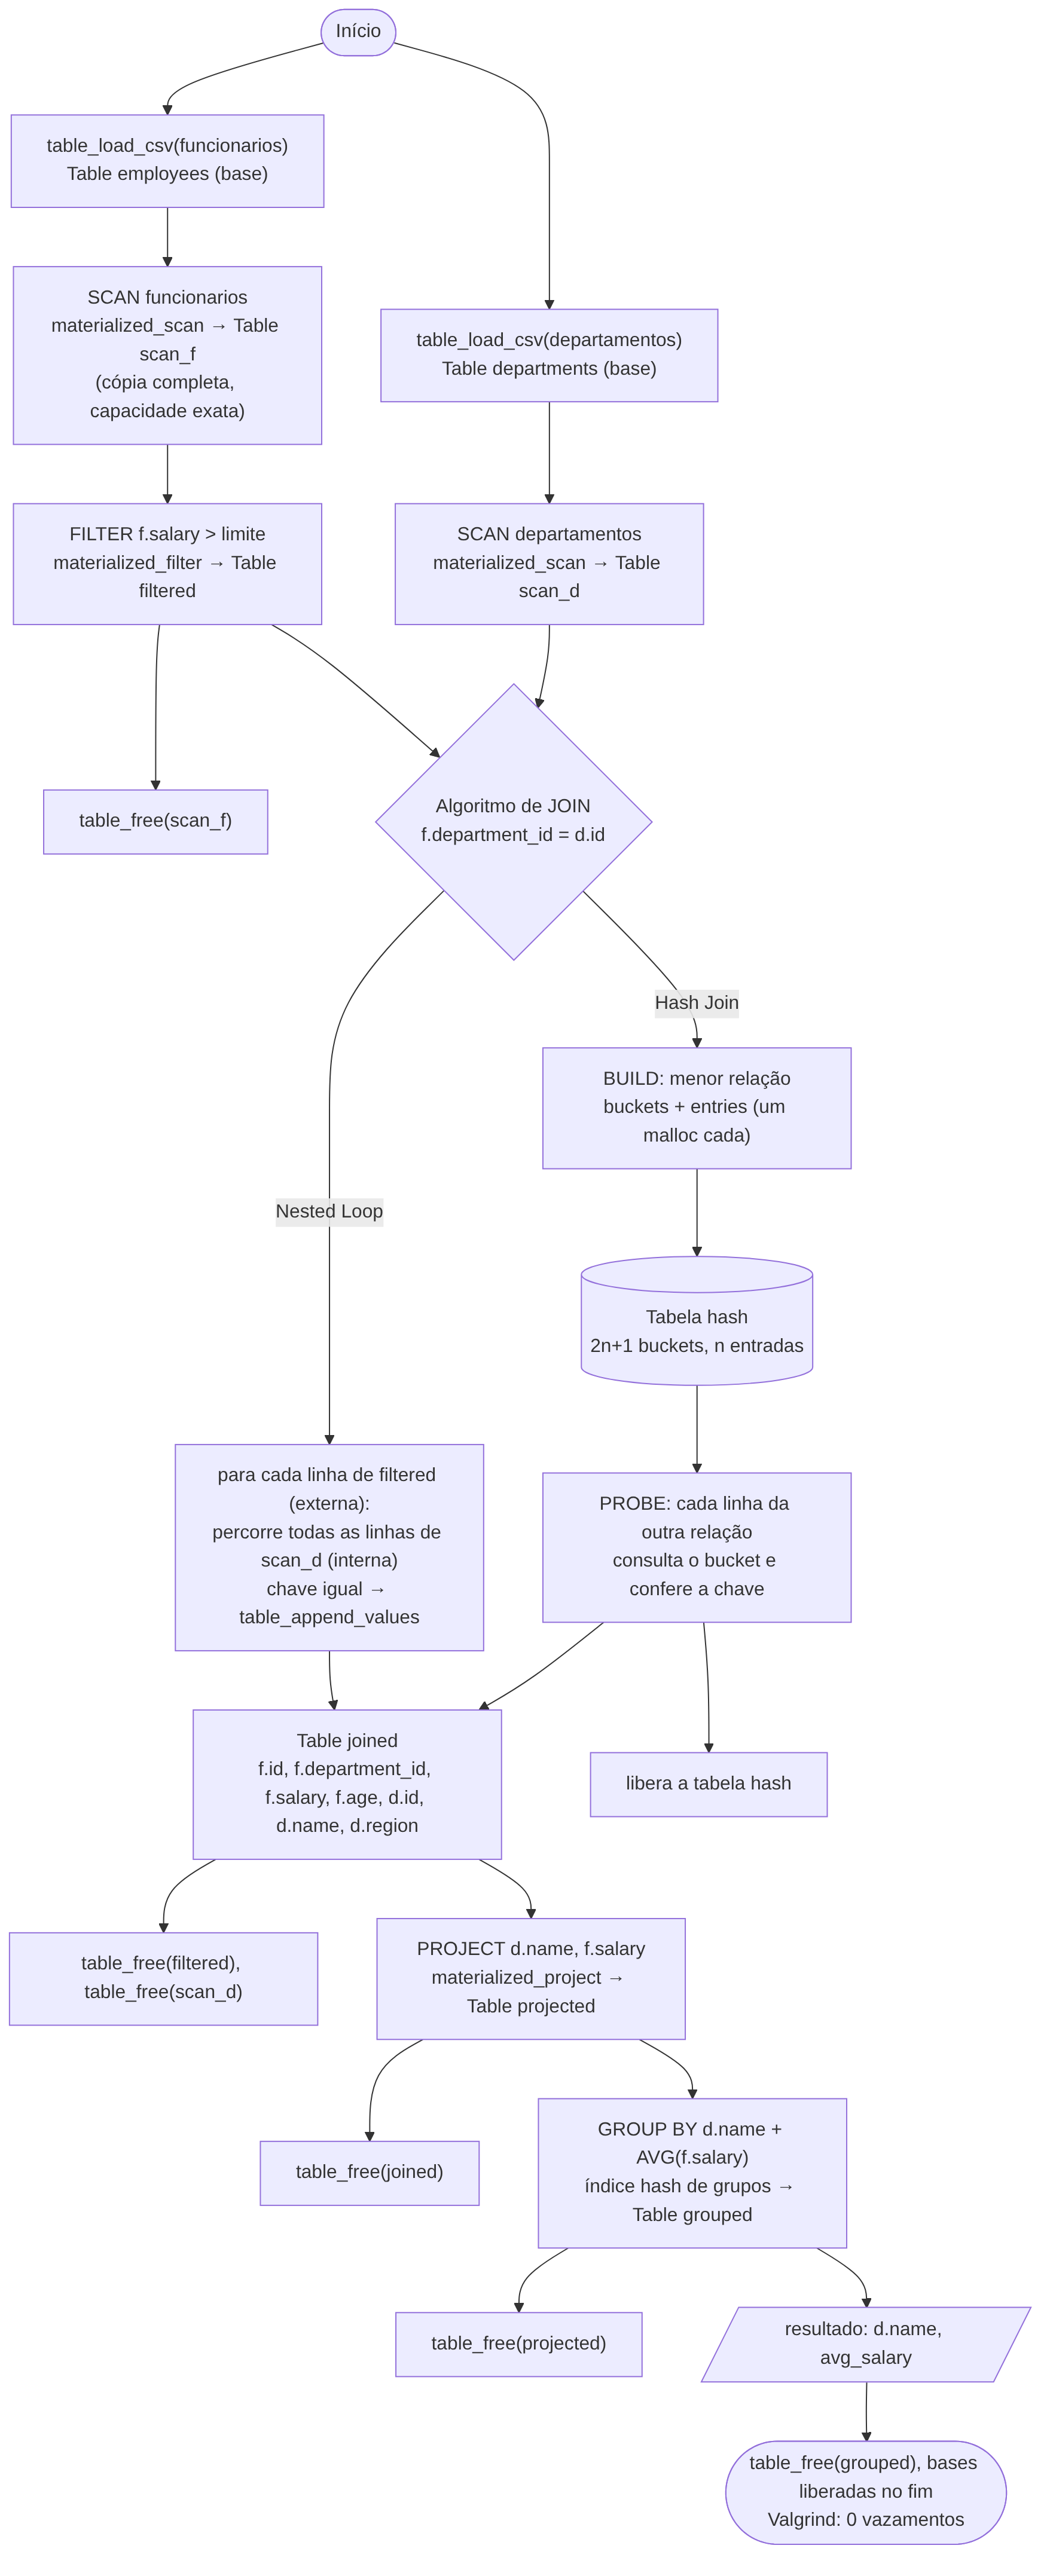
\includegraphics[height=0.88\textheight,keepaspectratio]{fluxograma-etapa3.png}
\caption{Fluxograma da consulta completa no modelo materializado.}
\label{fig:fluxo}
\end{figure}

\subsection{Suporte a múltiplas tabelas}
\texttt{funcionarios} e \texttt{departamentos} têm esquemas próprios e coexistem em memória como duas \texttt{Table} independentes (Tabela~\ref{tab:esquemas}).

\begin{table}[H]
\centering
\small
\begin{tabular}{@{}p{3.0cm}p{10.4cm}r@{}}
\toprule
Tabela & Esquema & Bytes por linha \\
\midrule
\texttt{funcionarios} & \texttt{id INT, department\_id INT, salary DOUBLE, age INT} & $4 \times 32 = 128$ \\
\texttt{departamentos} & \texttt{id INT, name STRING, region STRING} & $3 \times 32 = 96$ \\
saída do JOIN & \texttt{f.id, f.department\_id, f.salary, f.age, d.id, d.name, d.region} & $7 \times 32 = 224$ \\
saída do PROJECT & \texttt{d.name, f.salary} & $2 \times 32 = 64$ \\
\bottomrule
\end{tabular}
\caption{Esquemas das tabelas da consulta.}
\label{tab:esquemas}
\end{table}

Os pontos pedidos na seção 2 do enunciado ficam assim:
\begin{itemize}
    \item \textbf{Entradas do JOIN:} duas \texttt{const Table *}, a esquerda e a direita, com o nome da coluna de chave de cada uma e um alias (\texttt{"f"} e \texttt{"d"}). As entradas não são alteradas.
    \item \textbf{Esquema resultante:} \texttt{join\_schema} concatena as colunas da esquerda e da direita prefixadas pelo alias (\texttt{f.id}, \ldots, \texttt{d.region}). Nomes repetidos, como \texttt{id}, ficam inequívocos, e a ordem não depende de qual lado foi usado como BUILD.
    \item \textbf{Tuplas resultantes:} cada par com chaves iguais vira uma linha da saída, com os valores da esquerda seguidos dos da direita (\texttt{append\_joined\_row}). É um INNER JOIN: linhas sem par não aparecem e chaves repetidas geram todas as combinações.
    \item \textbf{Alocação e liberação:} o JOIN aloca a tabela de saída e, no Hash Join, a tabela hash. A tabela hash é liberada pelo próprio JOIN antes de retornar; a saída pertence ao chamador. Em erro, o JOIN libera a saída parcial e a tabela hash.
\end{itemize}

\section{Funcionamento dos operadores}

\subsection{SCAN, FILTER, PROJECT e AGGREGATE}
Os operadores da etapa 2 mantêm o contrato: entrada \texttt{const}, saída nova, retorno \texttt{1} ou \texttt{0}, saída parcial liberada em erro e métricas opcionais. Nesta etapa, o SCAN e o PROJECT passaram a reservar a capacidade exata (\texttt{input->size}) de uma vez, e todos leem e gravam pela representação compacta (Seção~\ref{sec:compacta}).

\subsection{Nested Loop Join}
\texttt{materialized\_nested\_loop\_join} usa a entrada esquerda como relação externa e a direita como relação interna. As duas já chegam materializadas. Para cada linha externa, o operador percorre todas as linhas internas e compara as chaves com \texttt{value\_equals}:
\par\medskip\noindent\begin{minipage}{\linewidth}
\begin{lstlisting}[language=C]
for (i = 0; i < left->size; ++i) {
    const Value *outer = table_row_const(left, i);
    for (j = 0; j < right->size; ++j) {
        const Value *inner = table_row_const(right, j);
        if (value_equals(&outer[left_index], &inner[right_index]) &&
            !append_joined_row(output, left, outer, right, inner)) {
            table_free(output);
            return 0;
        }
    }
    comparisons += right->size;
}
\end{lstlisting}
\end{minipage}\par\medskip
O custo é de $|R| \times |S|$ comparações, e a memória adicional é só a da saída. Não há fase de construção, então \texttt{build\_time\_ms} vale zero. Nas métricas, \texttt{build\_rows} é a relação interna (percorrida de novo a cada linha externa) e \texttt{probe\_rows} é a externa. Na consulta, a externa é \texttt{funcionarios} filtrado e a interna é \texttt{departamentos}.

\subsection{Hash Join: BUILD e PROBE}
\texttt{materialized\_hash\_join} escolhe como BUILD a menor relação (a esquerda, em caso de empate) e usa a outra como PROBE. A tabela hash é formada por dois vetores alocados de uma vez: \texttt{heads}, com $2n+1$ buckets, e \texttt{entries}, com uma entrada \texttt{\{row\_index, next\}} por linha de BUILD, encadeadas por índice. Ela ocupa $(2n+1) \times 8 + n \times 16$ bytes.
\par\medskip\noindent\begin{minipage}{\linewidth}
\begin{lstlisting}[language=C]
/* BUILD: one bucket array plus one entry per BUILD row, both allocated up front. */
table->bucket_count = build->size * 2 + 1;
table->heads = malloc(table->bucket_count * sizeof(*table->heads));
table->entries = malloc(build->size * sizeof(*table->entries));
for (i = 0; i < table->bucket_count; ++i) table->heads[i] = HASH_CHAIN_END;
for (i = 0; i < build->size; ++i) {
    size_t bucket = value_hash(table_cell(build, i, key)) % table->bucket_count;
    table->entries[i].row_index = i;
    table->entries[i].next = table->heads[bucket];
    table->heads[bucket] = i;
}
\end{lstlisting}
\end{minipage}\par\medskip
No PROBE, cada linha calcula o hash da sua chave, percorre a cadeia do bucket, confere a igualdade (a cadeia mistura colisões e chaves repetidas) e grava a linha combinada na ordem \texttt{f} seguida de \texttt{d}:
\par\medskip\noindent\begin{minipage}{\linewidth}
\begin{lstlisting}[language=C]
for (i = 0; i < probe->size && hash.bucket_count != 0; ++i) {
    const Value *probe_row = table_row_const(probe, i);
    const Value *probe_value = &probe_row[probe_key];
    size_t entry = hash.heads[value_hash(probe_value) % hash.bucket_count];
    while (entry != HASH_CHAIN_END) {
        const Value *build_row = table_row_const(build, hash.entries[entry].row_index);
        ++comparisons;
        if (value_equals(&build_row[build_key], probe_value)) {
            /* append f.* followed by d.* to the output table */
        }
        entry = hash.entries[entry].next;
    }
}
\end{lstlisting}
\end{minipage}\par\medskip
O tempo esperado é $O(|R| + |S| + \text{resultado})$, e a memória adicional é $O(\min(|R|,|S|))$ para a tabela hash, mais a saída. A tabela hash é liberada antes de o operador retornar, e as métricas guardam o seu tamanho.

A Tabela~\ref{tab:hjmodelo} responde aos pontos da seção 4 do enunciado sobre o Hash Join em cada modelo.

\begin{table}[H]
\centering
\small
\begin{tabular}{@{}p{2.9cm}p{6.5cm}p{6.6cm}@{}}
\toprule
Pergunta & Modelo materializado (medido) & Pipeline e vetorizado (esperado, não medido) \\
\midrule
Que partes podem funcionar em pipeline? & Nenhuma: cada operador termina antes do próximo. O PROBE processa linha a linha, mas grava tudo numa tabela & O PROBE e o que vem depois (PROJECT, acumulação do GROUP BY) podem consumir as linhas à medida que são produzidas \\
Que etapas precisam esperar? & Todas esperam a anterior. O BUILD espera o SCAN de departamentos; o PROBE espera o BUILD e o FILTER & O BUILD precisa consumir a relação inteira antes do primeiro PROBE, em qualquer modelo. O GROUP BY só emite no fim \\
Que estruturas intermediárias são mantidas? & Tabelas de SCAN, FILTER, JOIN e PROJECT, mais a tabela hash durante o JOIN & Só a tabela hash e o estado dos grupos; no vetorizado, também um lote por operador \\
Que etapas consomem mais memória? & A saída do JOIN (224 bytes por linha) e a do FILTER, vivas ao mesmo tempo. A tabela hash é pequena: 31\,KiB com 1\,000 departamentos e 3,1\,MiB com 100\,000 & A tabela hash do BUILD passa a ser o maior consumidor \\
Como o modelo interfere em BUILD e PROBE? & O BUILD recebe a relação completa sem custo extra, porque ela já está materializada. A saída do PROBE é materializada inteira: com 10 milhões de funcionários, 1,75\,GiB reservados & O BUILD continua igual. O PROBE deixa de produzir uma tabela; o custo por linha passa a incluir as chamadas \texttt{next()} (pipeline) ou é amortizado por lote (vetorizado) \\
\bottomrule
\end{tabular}
\caption{Hash Join e modelo de execução.}
\label{tab:hjmodelo}
\end{table}

\subsection{GROUP BY e AGGREGATE}
\texttt{materialized\_group\_by} aceita uma ou mais colunas de agrupamento (inteiras ou texto) e uma função (\texttt{COUNT}, \texttt{SUM}, \texttt{MIN}, \texttt{MAX} ou \texttt{AVG}). A saída é uma tabela com as colunas de grupo seguidas de uma coluna \texttt{DOUBLE} com o resultado, e os grupos ficam na ordem da primeira ocorrência. A busca linear pelos grupos da versão anterior ($O(n \times g)$) foi trocada por um índice hash de grupos (\texttt{heads}, \texttt{next} e estados, que dobram de tamanho quando enchem), com tempo esperado $O(n)$. A mudança foi necessária para o experimento de BUILD: com 100\,000 departamentos, a busca linear faria até 600 mil $\times$ 100 mil comparações só no GROUP BY. O índice e os estados são liberados antes de o operador retornar. A consulta isolada \texttt{SELECT department\_id, AVG(salary) FROM funcionarios GROUP BY department\_id} é coberta pelos testes, e a integrada aparece no fim do plano.

\section{Decisões de implementação}

\subsection{Tabela compacta}\label{sec:compacta}
Na etapa 2, cada linha ocupava 16 valores de 136 bytes (2176 bytes), qualquer que fosse o esquema. Assim, só a tabela base de 10 milhões de funcionários ocuparia cerca de 20\,GiB, e a cópia do SCAN mais 20\,GiB, numa máquina de 16\,GiB. A linha compacta, já listada como otimização no relatório da etapa 2, foi implementada:
\par\medskip\noindent\begin{minipage}{\linewidth}
\begin{lstlisting}[language=C]
typedef struct {
    Schema schema;
    Value *values;   /* size * schema.column_count valores, linha a linha */
    size_t size;
    size_t capacity;
} Table;
\end{lstlisting}
\end{minipage}\par\medskip
\begin{itemize}
    \item A linha $i$ começa em \texttt{values + i * column\_count}, e o acesso é feito por \texttt{table\_cell}, \texttt{table\_row\_const} e \texttt{table\_row\_mut} (\texttt{static inline} em \texttt{table.h}).
    \item \texttt{Row} continua existindo, mas só como tupla de montagem na pilha; \texttt{table\_append} copia apenas as colunas do esquema.
    \item \texttt{VALUE\_STRING\_MAX\_LEN} caiu de 128 para 24, e \texttt{sizeof(Value)} de 136 para 32 bytes. O leitor de CSV passou a rejeitar strings com 24 caracteres ou mais, em vez de truncar sem avisar. Os nomes gerados (\texttt{department\_100000}) têm até 17.
\end{itemize}
Com isso, \texttt{funcionarios} passou de 2176 para 128 bytes por linha, 17 vezes menos.

\subsection{Outras decisões}
\begin{itemize}
    \item \textbf{Capacidade exata.} SCAN e PROJECT reservam \texttt{input->size} linhas de uma vez, e o leitor de CSV ajusta o vetor ao tamanho final (\texttt{table\_shrink\_to\_fit}). FILTER, JOIN e GROUP BY não conhecem o tamanho da saída e continuam dobrando a capacidade.
    \item \textbf{BUILD na menor relação}, como pede o enunciado, decidido em tempo de execução pelo número de linhas das entradas já materializadas.
    \item \textbf{Tabela hash em dois vetores}, em vez de um \texttt{malloc} por nó: duas alocações por JOIN, liberação simples e melhor localidade.
    \item \textbf{Função de hash única} (\texttt{value\_hash}, djb2 sobre os bytes do valor seguida de uma etapa de mistura), usada pelo JOIN e pelo GROUP BY. Inteiros e \texttt{double} de mesmo valor têm o mesmo hash, coerente com \texttt{value\_equals}.
    \item \textbf{Ordem do plano.} JOIN $\rightarrow$ PROJECT $\rightarrow$ GROUP BY, como no pipeline conceitual do enunciado. A versão anterior do \texttt{main.c} agrupava antes de projetar.
    \item \textbf{Liberação antecipada no benchmark.} Cada intermediário é liberado assim que o consumidor termina. O pico de memória passa a ser o maior conjunto de tabelas vivas ao mesmo tempo, e não a soma de todas.
\end{itemize}

\section{Gerenciamento de memória}\label{sec:memoria}

\subsection{Quem aloca e quem libera}
A Tabela~\ref{tab:posse} resume a posse de cada recurso.

\begin{table}[H]
\centering
\small
\begin{tabular}{@{}p{4.2cm}p{3.6cm}p{2.9cm}p{4.6cm}@{}}
\toprule
Recurso & Quem aloca & Dono & Quem libera \\
\midrule
Vetor de valores das tabelas base & \texttt{table\_load\_csv} & chamador & \texttt{table\_free}, no fim \\
Saída de SCAN, FILTER, PROJECT, JOIN e GROUP BY & o operador & o chamador (\texttt{output}) & o chamador, depois do último consumidor \\
Tabela hash (\texttt{heads}, \texttt{entries}) & \texttt{hash\_build} & o Hash Join & \texttt{hash\_table\_free}, antes de retornar (também em erro) \\
Índice de grupos & \texttt{materialized\_\allowbreak group\_by} & o GROUP BY & \texttt{group\_index\_free}, antes de retornar (também em erro) \\
\texttt{Row} de montagem & pilha & a função & fim do escopo \\
Strings & dentro do \texttt{Value} & a tabela & junto com o vetor de valores \\
\bottomrule
\end{tabular}
\caption{Alocação e liberação de memória.}
\label{tab:posse}
\end{table}

No benchmark, a ordem de liberação é: \texttt{scan\_f} depois do FILTER; \texttt{filtered} e \texttt{scan\_d} depois do JOIN; \texttt{joined} depois do PROJECT; \texttt{projected} depois do GROUP BY. Não há buffer reutilizado entre operadores. Ponteiros obtidos por \texttt{table\_cell} e similares valem até o próximo crescimento da tabela ou até \texttt{table\_free}, e nenhum operador guarda ponteiro de entrada depois de retornar. \texttt{input == output} continua sendo rejeitado.

A métrica \texttt{memory\_bytes} mede a capacidade reservada (capacidade $\times$ bytes por linha). O pico de RSS do processo (\texttt{VmHWM}, que inclui as tabelas base) pode ficar abaixo da soma reservada, porque páginas reservadas e nunca escritas não ocupam memória física. Por isso os experimentos reportam as duas medidas.

\subsection{Validação com Valgrind}\label{sec:valgrind}
O Valgrind Memcheck \cite{valgrind} foi executado no código final desta etapa (Tabela~\ref{tab:valgrind}); os logs completos estão em \texttt{results/validacao/}. \texttt{make sanitize} (AddressSanitizer e UndefinedBehaviorSanitizer) terminou com \texttt{all materialized tests passed}. A diferença de 2 alocações entre os dois JOINs no benchmark corresponde aos dois vetores da tabela hash.

\begin{table}[H]
\centering
\small
\begin{tabular}{@{}lrrrrr@{}}
\toprule
Programa & Alocações & Liberações & Bytes alocados & Em uso & Erros \\
\midrule
\texttt{test\_materialized} & 218 & 218 & 12\,881\,115 & 0 & 0 \\
\texttt{miniquery} (dataset versionado) & 26 & 26 & 38\,168 & 0 & 0 \\
\texttt{miniquery\_bench}, HJ, 10 mil linhas & 74 & 74 & 13\,548\,048 & 0 & 0 \\
\texttt{miniquery\_bench}, NLJ, 10 mil linhas & 72 & 72 & 13\,516\,040 & 0 & 0 \\
\bottomrule
\end{tabular}
\caption{Resultados do Valgrind Memcheck.}
\label{tab:valgrind}
\end{table}

\section{Instrumentação}
A estrutura \texttt{JoinMetrics} registra o que a seção 5 do enunciado pede, e alguns campos extras (Tabela~\ref{tab:metricas}). \texttt{batch\_size} e \texttt{batches\_processed} são do modelo vetorizado e não se aplicam aqui. \texttt{QueryMetrics} (SCAN, FILTER, PROJECT e GROUP BY) registra \texttt{rows\_in}, \texttt{rows\_out}, \texttt{memory\_bytes} e \texttt{time\_ms}. O benchmark mede ainda o tempo de parede da consulta inteira com \texttt{timespec\_get} e o pico de RSS do processo.

\begin{table}[H]
\centering
\small
\begin{tabular}{@{}p{6.4cm}p{10.0cm}@{}}
\toprule
Campo & Significado \\
\midrule
\texttt{build\_rows}, \texttt{probe\_rows} & Linhas de BUILD e PROBE (no Nested Loop, relação interna e externa) \\
\texttt{rows\_out} & Linhas produzidas pelo JOIN \\
\texttt{build\_time\_ms}, \texttt{probe\_time\_ms}, \texttt{total\_time\_ms} & Tempo de CPU (\texttt{clock()}) de cada fase e do operador inteiro \\
\texttt{memory\_bytes} & Tabela hash mais a saída reservada \\
\texttt{hash\_table\_entries}, \texttt{hash\_table\_bytes} & Entradas e bytes da tabela hash \\
\texttt{hash\_buckets}, \texttt{key\_comparisons}, \texttt{output\_bytes}, \texttt{build\_is\_left} & Extras: buckets, comparações de chave executadas, bytes da saída e lado escolhido para BUILD \\
\bottomrule
\end{tabular}
\caption{Métricas do JOIN.}
\label{tab:metricas}
\end{table}

A saída do \texttt{./miniquery} sobre o dataset versionado (8 funcionários e 5 departamentos) segue o formato do enunciado; o bloco \texttt{[NESTED\_LOOP\_JOIN]} sai antes, com \texttt{key\_comparisons=25} ($5 \times 5$). Os tempos variam entre execuções.
\par\medskip\noindent\begin{minipage}{\linewidth}
\begin{lstlisting}
SCAN f: 8 linhas | SCAN d: 5 linhas | FILTER salary > 5000.00: 5 linhas

[HASH_JOIN]
build_rows=5
probe_rows=5
hash_table_entries=5
hash_table_bytes=168
build_time_ms=0.001
probe_time_ms=0.002
total_time_ms=0.004
rows_out=6
memory_bytes=3752
key_comparisons=6
\end{lstlisting}
\end{minipage}\par\medskip

\section{Testes automatizados}\label{sec:testes}
\texttt{make test} compila a suíte com \texttt{-std=c11 -Wall -Wextra -Wpedantic -Werror -O2}, roda 14 grupos de teste e termina com \texttt{all materialized tests passed}:
\begin{itemize}
    \item \textbf{Etapa 2:} CSV e esquema, cópia independente do SCAN, FILTER, PROJECT, agregações e pipeline completo.
    \item \textbf{JOIN:} aliases e esquema resultante, chaves repetidas, chave sem par, os dois lados possíveis de BUILD, entrada vazia e equivalência por multiconjunto entre Nested Loop e Hash Join em $2\,000 \times 300$ linhas pseudoaleatórias, com chaves repetidas e chaves sem par.
    \item \textbf{Métricas:} \texttt{key\_comparisons} $= |R| \times |S|$ no Nested Loop, tamanho exato da tabela hash e \texttt{memory\_bytes} igual a hash mais saída.
    \item \textbf{GROUP BY:} as cinco funções por grupo, chave inteira e texto, e 20\,000 linhas em 5\,000 grupos, para forçar o crescimento do índice e conferir a ordem e as médias.
    \item \textbf{Armazenamento compacto:} bytes por linha, capacidade exata e rejeição de string longa demais no CSV.
    \item \textbf{Consulta completa} na ordem do enunciado, com os valores esperados (\texttt{engineering 6500}, \texttt{finance 7600}, \texttt{finance-remote 7600}, \texttt{operations 9100}).
\end{itemize}
Além disso, os experimentos conferem a cada configuração que os dois algoritmos devolvem o mesmo número de linhas e a mesma soma das médias por grupo. Não houve divergência.

\section{Experimentos}\label{sec:experimentos}

\subsection{Configuração utilizada}
\begin{table}[H]
\centering
\small
\begin{tabular}{@{}p{3.0cm}p{13.4cm}@{}}
\toprule
Item & Valor \\
\midrule
CPU & Intel Xeon (KVM), 8 CPUs lógicas; L1d 48\,KiB e L2 2\,MiB por núcleo; L3 320\,MiB \\
Memória & 15,6\,GiB (12,7\,GiB disponíveis no início) \\
Sistema & Debian GNU/Linux 13 (trixie), kernel 6.12, máquina virtual compartilhada \\
Compilador & GCC 14.2.0, \texttt{-std=c11 -Wall -Wextra -Wpedantic -Werror -O2} \\
Execução & 1 thread, sequencial, um processo por configuração (dataset, algoritmo, limite) \\
Repetições & 1 de aquecimento (descartada) e 5 medidas, com mediana; sem aquecimento no Nested Loop acima de $5 \times 10^9$ comparações \\
Data & 11/11/2026; detalhes em \texttt{results/ambiente.txt} \\
\bottomrule
\end{tabular}
\caption{Ambiente dos experimentos.}
\label{tab:ambiente}
\end{table}

Os datasets base são carregados uma vez por processo, fora do tempo medido, e cada repetição executa a consulta inteira de novo, com alocações novas. A máquina é virtual e compartilhada, então há ruído: a mesma configuração (1 milhão de funcionários, 1\,000 departamentos, \texttt{salary > 5000}) medida em dois processos diferentes deu 254,5 e 250,8\,ms com Hash Join e 1\,821,7 e 1\,998,0\,ms com Nested Loop, cerca de 10\% de diferença.

\subsection{Datasets}
\texttt{bench/generate\_data.py} gera dados determinísticos (semente 2026). Em \texttt{departamentos}, os ids vão de 1 a $D$, com \texttt{name = department\_<id>} e \texttt{region = region\_<id \% 5>}. Em \texttt{funcionarios}, \texttt{department\_id} é uniforme em $1..D$ (toda linha tem par), \texttt{salary} é uniforme em $[1000, 11000)$ e \texttt{age} em $18..70$. Assim, \texttt{salary > t} mantém cerca de $(11000 - t)/10000$ das linhas.

\begin{table}[H]
\centering
\small
\begin{tabular}{@{}lrr@{}}
\toprule
Arquivo & Linhas & Tamanho \\
\midrule
\texttt{funcionarios\_10k\_d1k.csv} & 10\,000 & 0,2\,MB \\
\texttt{funcionarios\_100k\_d1k.csv} & 100\,000 & 2,1\,MB \\
\texttt{funcionarios\_1m\_d1k.csv} (e \texttt{\_d100}, \texttt{\_d10k}, \texttt{\_d100k}) & 1\,000\,000 cada & 21 a 24\,MB \\
\texttt{funcionarios\_5m\_d1k.csv} & 5\,000\,000 & 114\,MB \\
\texttt{funcionarios\_10m\_d1k.csv} & 10\,000\,000 & 229\,MB \\
\texttt{departamentos\_100.csv} a \texttt{departamentos\_100k.csv} & 100 a 100\,000 & 2,6\,KB a 3,2\,MB \\
\bottomrule
\end{tabular}
\caption{Datasets dos experimentos.}
\label{tab:datasets}
\end{table}

\texttt{results/datasets.csv} registra o tamanho e o SHA-256 de cada arquivo, e \texttt{make experiments} recria exatamente os mesmos bytes. Os arquivos de 5 e 10 milhões passam dos limites de um repositório comum (o GitHub recusa arquivos acima de 100\,MB). Por isso ficam versionados só os datasets pequenos, em \texttt{data/experimentos/}, além do gerador com a semente. Compactado, o arquivo de 10 milhões tem 93\,MB com gzip e 69\,MB com xz.

\subsection{Consulta, algoritmos e métricas}
Todas as medições usam a consulta completa da seção 7 do enunciado, mudando só o limite do FILTER. O plano é \texttt{SCAN f $\rightarrow$ FILTER $\rightarrow$ JOIN $\leftarrow$ SCAN d $\rightarrow$ PROJECT (d.name, f.salary) $\rightarrow$ GROUP BY/AVG}, executado com Nested Loop Join (externa: \texttt{funcionarios} filtrado; interna: \texttt{departamentos}) e com Hash Join (BUILD: a menor entrada, que foi sempre \texttt{departamentos}; PROBE: \texttt{funcionarios} filtrado).

Por repetição são registrados (\texttt{results/raw/*.csv}): linhas de cada operador, tempo de CPU de cada operador (SCAN f, SCAN d, FILTER, BUILD, PROBE, JOIN, PROJECT e GROUP BY), tempo de parede da consulta, comparações de chave, entradas e bytes da tabela hash, bytes reservados por intermediário, pico de intermediários vivos, pico de RSS e uma soma de verificação das médias. Nas tabelas a seguir, ``Consulta'' é a mediana do tempo de parede da consulta inteira, ``Pico interm.'' é o maior conjunto de tabelas intermediárias vivas ao mesmo tempo e ``Pico RSS'' é a memória física máxima do processo, incluindo as tabelas base. Todos os tempos estão em milissegundos.

\subsection{Cardinalidade}
Com 1\,000 departamentos e \texttt{salary > 5000} (cerca de 60\% das linhas), a quantidade de funcionários variou de 10 mil a 10 milhões. Todas as cardinalidades pedidas foram executadas, inclusive 10 milhões com Nested Loop ($6 \times 10^9$ comparações, cerca de 20\,s por repetição). As Tabelas~\ref{tab:cardinalidade-tempo} a \ref{tab:cardinalidade-mem} e as Figuras~\ref{fig:card-tempo} a \ref{fig:card-ops} trazem os resultados (HJ: Hash Join; NLJ: Nested Loop Join).

\begin{table}[H]
\centering
\footnotesize
\setlength{\tabcolsep}{3.5pt}
\begin{tabular}{@{}rlrrrrrrr@{}}
\toprule
Funcionários & Alg. & Linhas PROBE & Comparações & BUILD & PROBE & JOIN & Consulta & min--max \\
\midrule
10\,000 & HJ & 5\,862 & 8\,565 & 0,010 & 0,7 & 0,7 & \textbf{2,0} & 1,9--2,0 \\
10\,000 & NLJ & 5\,862 & 5\,862\,000 & 0,000 & 17,5 & 17,5 & \textbf{19,0} & 18,4--23,6 \\
\addlinespace[2pt]
100\,000 & HJ & 60\,051 & 88\,121 & 0,016 & 9,6 & 9,6 & \textbf{29,3} & 27,8--34,0 \\
100\,000 & NLJ & 60\,051 & 60\,051\,000 & 0,000 & 168,4 & 168,4 & \textbf{185,0} & 181,2--195,6 \\
\addlinespace[2pt]
1\,000\,000 & HJ & 600\,178 & 879\,899 & 0,027 & 71,6 & 71,6 & \textbf{254,5} & 246,0--315,4 \\
1\,000\,000 & NLJ & 600\,178 & 600\,178\,000 & 0,000 & 1\,645,6 & 1\,645,6 & \textbf{1\,821,7} & 1\,786,6--1\,971,6 \\
\addlinespace[2pt]
5\,000\,000 & HJ & 3\,000\,405 & 4\,396\,861 & 0,029 & 367,6 & 367,6 & \textbf{1\,290,3} & 1\,221,3--1\,415,8 \\
5\,000\,000 & NLJ & 3\,000\,405 & 3\,000\,405\,000 & 0,000 & 8\,482,0 & 8\,482,0 & \textbf{9\,399,0} & 9\,303,7--9\,632,0 \\
\addlinespace[2pt]
10\,000\,000 & HJ & 5\,999\,764 & 8\,794\,780 & 0,027 & 741,2 & 741,2 & \textbf{2\,711,9} & 2\,656,2--2\,869,3 \\
10\,000\,000 & NLJ & 5\,999\,764 & 5\,999\,764\,000 & 0,000 & 17\,773,9 & 17\,773,9 & \textbf{19\,929,8} & 19\,323,4--20\,357,6 \\
\bottomrule
\end{tabular}
\caption{Experimento de cardinalidade: linhas, comparações e tempos (ms, mediana de 5 repetições).}
\label{tab:cardinalidade-tempo}
\end{table}
\begin{table}[H]
\centering
\footnotesize
\setlength{\tabcolsep}{3.5pt}
\begin{tabular}{@{}rlrrrrrrrr@{}}
\toprule
Funcionários & Alg. & SCAN f & SCAN d & FILTER & JOIN & PROJECT & GROUP BY & Soma & JOIN/soma \\
\midrule
10\,000 & HJ & 0,3 & 0,0 & 0,4 & 0,7 & 0,1 & 0,4 & 1,9 & 36\% \\
10\,000 & NLJ & 0,4 & 0,0 & 0,4 & 17,5 & 0,2 & 0,4 & 18,9 & 93\% \\
\addlinespace[2pt]
100\,000 & HJ & 6,4 & 0,0 & 5,4 & 9,6 & 2,7 & 3,6 & 28,1 & 34\% \\
100\,000 & NLJ & 5,7 & 0,0 & 5,2 & 168,4 & 2,5 & 2,7 & 184,1 & 91\% \\
\addlinespace[2pt]
1\,000\,000 & HJ & 57,5 & 0,0 & 48,9 & 71,6 & 37,1 & 25,4 & 245,4 & 29\% \\
1\,000\,000 & NLJ & 55,6 & 0,0 & 49,7 & 1\,645,6 & 36,3 & 25,4 & 1\,812,8 & 91\% \\
\addlinespace[2pt]
5\,000\,000 & HJ & 282,9 & 0,0 & 289,2 & 367,6 & 181,8 & 127,8 & 1\,247,5 & 29\% \\
5\,000\,000 & NLJ & 287,5 & 0,0 & 249,6 & 8\,482,0 & 187,4 & 126,2 & 9\,337,2 & 91\% \\
\addlinespace[2pt]
10\,000\,000 & HJ & 580,8 & 0,0 & 634,7 & 741,2 & 362,7 & 257,8 & 2\,610,9 & 28\% \\
10\,000\,000 & NLJ & 727,1 & 0,0 & 565,7 & 17\,773,9 & 432,2 & 250,2 & 19\,808,5 & 90\% \\
\bottomrule
\end{tabular}
\caption{Experimento de cardinalidade: tempo de CPU por operador (ms, mediana).}
\label{tab:cardinalidade-ops}
\end{table}
\begin{table}[H]
\centering
\footnotesize
\setlength{\tabcolsep}{3.5pt}
\begin{tabular}{@{}rrrrrrrrr@{}}
\toprule
Funcionários & SCAN f+d & FILTER & JOIN (saída) & Hash (KiB) & PROJECT & Total & Pico interm. & Pico RSS \\
\midrule
10\,000 & 1,3 & 1,0 & 1,8 & 31,3 & 0,4 & 4,6 & 2,9 & 6,6 \\
100\,000 & 12,3 & 8,0 & 14,0 & 31,3 & 3,7 & 38,1 & 22,1 & 50,0 \\
1\,000\,000 & 122,2 & 128,0 & 224,0 & 31,3 & 36,6 & 510,9 & 352,1 & 325,5 \\
5\,000\,000 & 610,4 & 512,0 & 896,0 & 31,3 & 183,1 & 2\,201,7 & 1\,408,1 & 1\,619,6 \\
10\,000\,000 & 1\,220,8 & 1\,024,0 & 1\,792,0 & 31,3 & 366,2 & 4\,403,1 & 2\,816,1 & 3\,236,7 \\
\bottomrule
\end{tabular}
\caption{Experimento de cardinalidade: memória com Hash Join (MiB, salvo indicação). ``Total'' é a soma reservada por todos os intermediários.}
\label{tab:cardinalidade-mem}
\end{table}
\begin{figure}[H]
\centering
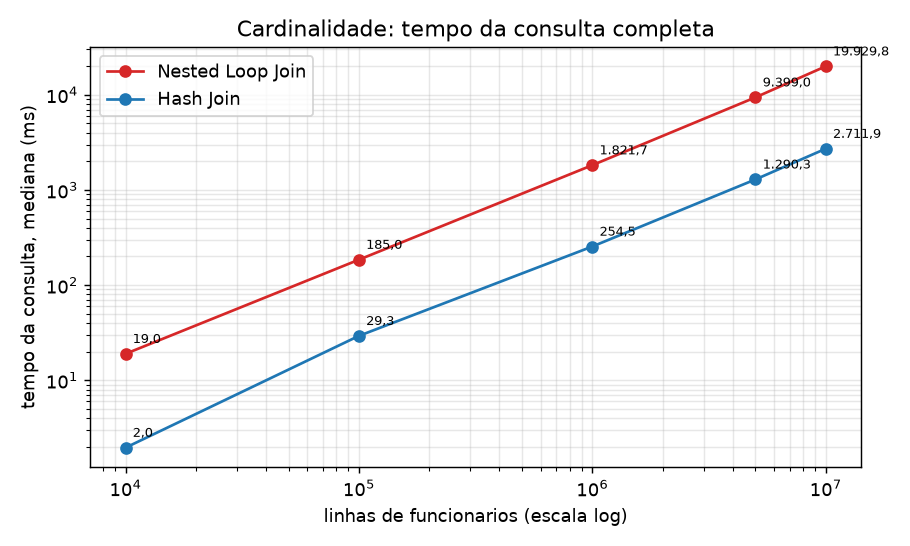
\includegraphics[width=0.82\linewidth]{cardinalidade_tempo.png}
\caption{Cardinalidade: tempo da consulta (mediana).}
\label{fig:card-tempo}
\end{figure}

\begin{figure}[H]
\centering
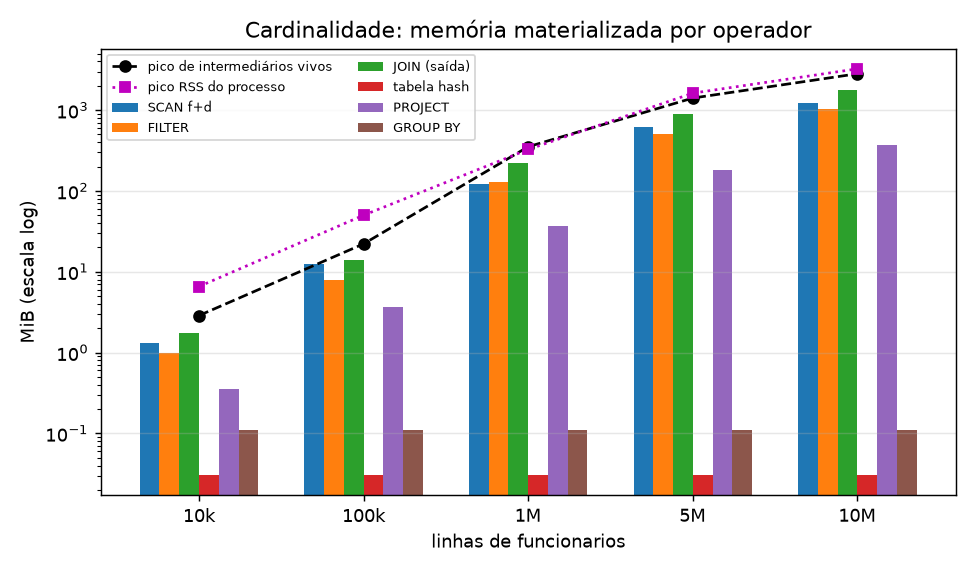
\includegraphics[width=0.82\linewidth]{cardinalidade_memoria.png}
\caption{Cardinalidade: memória reservada pelos intermediários e pico de RSS.}
\label{fig:card-mem}
\end{figure}

\begin{figure}[H]
\centering
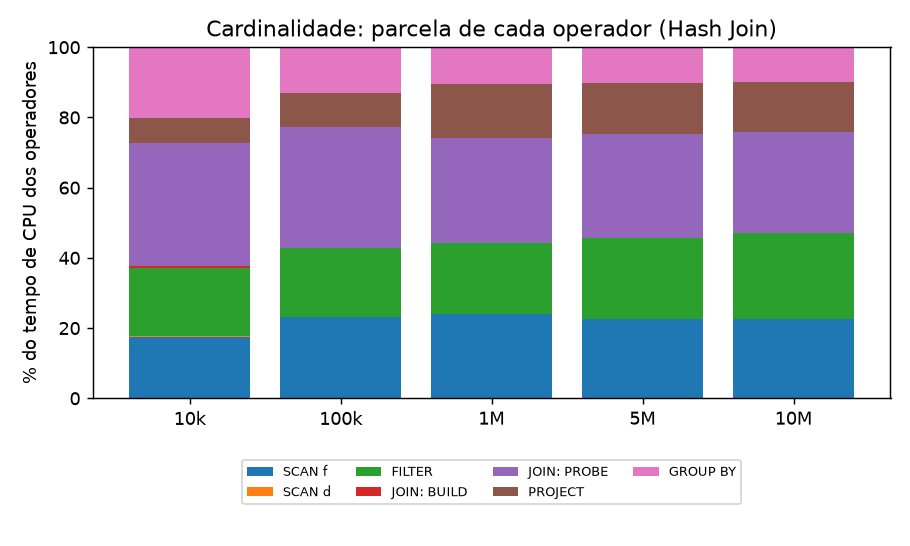
\includegraphics[width=0.82\linewidth]{cardinalidade_operadores.png}
\caption{Cardinalidade: parcela de cada operador no tempo.}
\label{fig:card-ops}
\end{figure}

O tempo cresce de forma linear com o número de funcionários nos dois algoritmos, porque o número de departamentos está fixo. O Nested Loop faz $|F'| \times 1\,000$ comparações (cerca de 3\,ns cada) e gasta de 90 a 93\% do tempo dos operadores no JOIN. O Hash Join faz cerca de 1,47 comparação por linha de PROBE e gasta de 28 a 36\% no JOIN. A diferença entre os dois fica estável em cerca de 7 vezes a partir de 100 mil linhas. A memória também cresce de forma linear: com 10 milhões, a consulta reserva 4,3\,GiB de intermediários para devolver 1\,000 grupos, e o pico de intermediários vivos chega a 2,75\,GiB durante o JOIN, quando a saída do FILTER e a do JOIN coexistem.

\subsection{Seletividade}
Com 1 milhão de funcionários e 1\,000 departamentos, os limites 10\,900, 10\,000, 6\,000 e 2\,000 mantêm 1, 10, 50 e 90\% das linhas. As seletividades medidas foram 0,98\%, 9,95\%, 50,0\% e 90,0\%.

\begin{table}[H]
\centering
\footnotesize
\setlength{\tabcolsep}{3.5pt}
\begin{tabular}{@{}rlrrrrrrr@{}}
\toprule
Seletividade & Alg. & Linhas PROBE & Comparações & BUILD & PROBE & JOIN & Consulta & min--max \\
\midrule
1,0\% & HJ & 9\,798 & 14\,244 & 0,023 & 1,1 & 1,2 & \textbf{80,6} & 78,5--82,1 \\
1,0\% & NLJ & 9\,798 & 9\,798\,000 & 0,000 & 35,0 & 35,0 & \textbf{128,9} & 103,6--150,4 \\
\addlinespace[2pt]
10,0\% & HJ & 99\,519 & 145\,589 & 0,024 & 12,1 & 12,2 & \textbf{104,6} & 103,0--124,8 \\
10,0\% & NLJ & 99\,519 & 99\,519\,000 & 0,000 & 275,7 & 275,7 & \textbf{375,8} & 370,9--455,9 \\
\addlinespace[2pt]
50,0\% & HJ & 500\,004 & 732\,986 & 0,027 & 66,3 & 66,3 & \textbf{220,4} & 217,7--233,3 \\
50,0\% & NLJ & 500\,004 & 500\,004\,000 & 0,000 & 1\,408,0 & 1\,408,0 & \textbf{1\,569,4} & 1\,520,7--1\,623,5 \\
\addlinespace[2pt]
90,0\% & HJ & 900\,002 & 1\,319\,626 & 0,026 & 106,5 & 106,6 & \textbf{324,9} & 321,6--328,5 \\
90,0\% & NLJ & 900\,002 & 900\,002\,000 & 0,000 & 2\,530,0 & 2\,530,0 & \textbf{2\,781,2} & 2\,729,0--3\,079,5 \\
\bottomrule
\end{tabular}
\caption{Experimento de seletividade: linhas, comparações e tempos (ms, mediana de 5 repetições).}
\label{tab:seletividade-tempo}
\end{table}
\begin{table}[H]
\centering
\footnotesize
\setlength{\tabcolsep}{3.5pt}
\begin{tabular}{@{}rlrrrrrrrr@{}}
\toprule
Seletividade & Alg. & SCAN f & SCAN d & FILTER & JOIN & PROJECT & GROUP BY & Soma & JOIN/soma \\
\midrule
1,0\% & HJ & 56,9 & 0,0 & 17,9 & 1,2 & 0,2 & 0,5 & 77,0 & 2\% \\
1,0\% & NLJ & 63,8 & 0,0 & 20,5 & 35,0 & 0,4 & 0,6 & 124,5 & 28\% \\
\addlinespace[2pt]
10,0\% & HJ & 56,2 & 0,0 & 23,9 & 12,2 & 3,8 & 5,1 & 101,4 & 12\% \\
10,0\% & NLJ & 59,9 & 0,0 & 25,0 & 275,7 & 4,2 & 4,5 & 372,5 & 74\% \\
\addlinespace[2pt]
50,0\% & HJ & 56,1 & 0,0 & 49,0 & 66,3 & 21,6 & 21,8 & 214,3 & 31\% \\
50,0\% & NLJ & 57,3 & 0,0 & 54,6 & 1\,408,0 & 20,6 & 21,4 & 1\,561,4 & 90\% \\
\addlinespace[2pt]
90,0\% & HJ & 55,9 & 0,0 & 60,1 & 106,6 & 53,8 & 37,6 & 313,6 & 34\% \\
90,0\% & NLJ & 61,0 & 0,0 & 64,8 & 2\,530,0 & 61,4 & 39,5 & 2\,763,1 & 92\% \\
\bottomrule
\end{tabular}
\caption{Experimento de seletividade: tempo de CPU por operador (ms, mediana).}
\label{tab:seletividade-ops}
\end{table}
\begin{table}[H]
\centering
\footnotesize
\setlength{\tabcolsep}{3.5pt}
\begin{tabular}{@{}rrrrrrrrr@{}}
\toprule
Seletividade & SCAN f+d & FILTER & JOIN (saída) & Hash (KiB) & PROJECT & Total & Pico interm. & Pico RSS \\
\midrule
1,0\% & 122,2 & 2,0 & 3,5 & 31,3 & 0,6 & 128,4 & 124,2 & 247,6 \\
10,0\% & 122,2 & 16,0 & 28,0 & 31,3 & 6,1 & 172,4 & 138,2 & 264,1 \\
50,0\% & 122,2 & 64,0 & 112,0 & 31,3 & 30,5 & 328,8 & 186,2 & 339,0 \\
90,0\% & 122,2 & 128,0 & 224,0 & 31,3 & 54,9 & 529,2 & 352,1 & 426,2 \\
\bottomrule
\end{tabular}
\caption{Experimento de seletividade: memória com Hash Join (MiB, salvo indicação). ``Total'' é a soma reservada por todos os intermediários.}
\label{tab:seletividade-mem}
\end{table}
\begin{figure}[H]
\centering
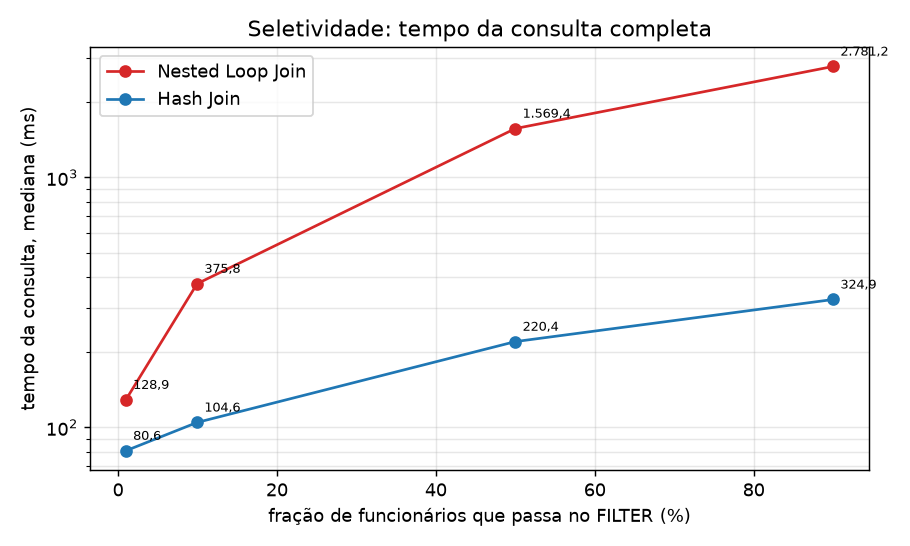
\includegraphics[width=0.82\linewidth]{seletividade_tempo.png}
\caption{Seletividade: tempo da consulta (mediana).}
\label{fig:sel-tempo}
\end{figure}

\begin{figure}[H]
\centering
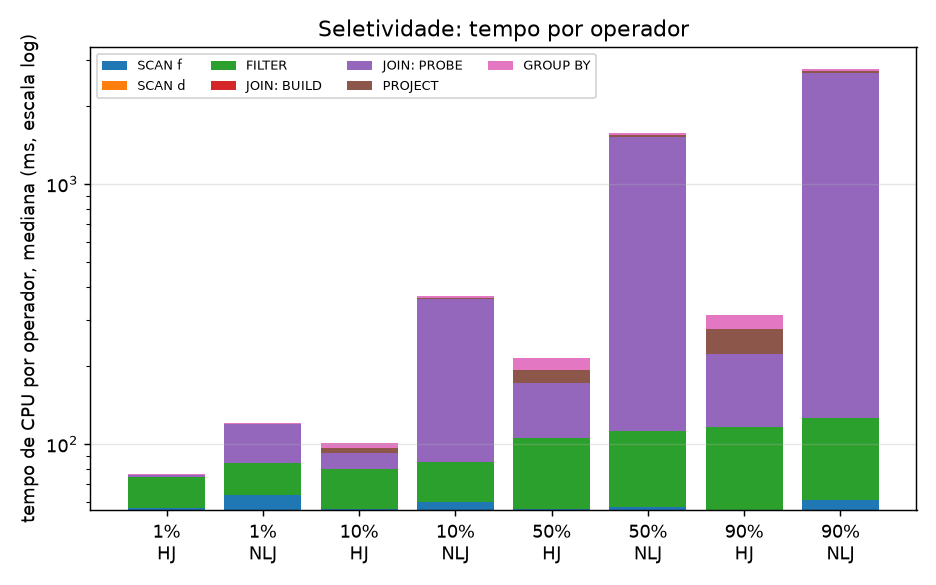
\includegraphics[width=0.82\linewidth]{seletividade_operadores.png}
\caption{Seletividade: tempo por operador.}
\label{fig:sel-ops}
\end{figure}

\begin{figure}[H]
\centering
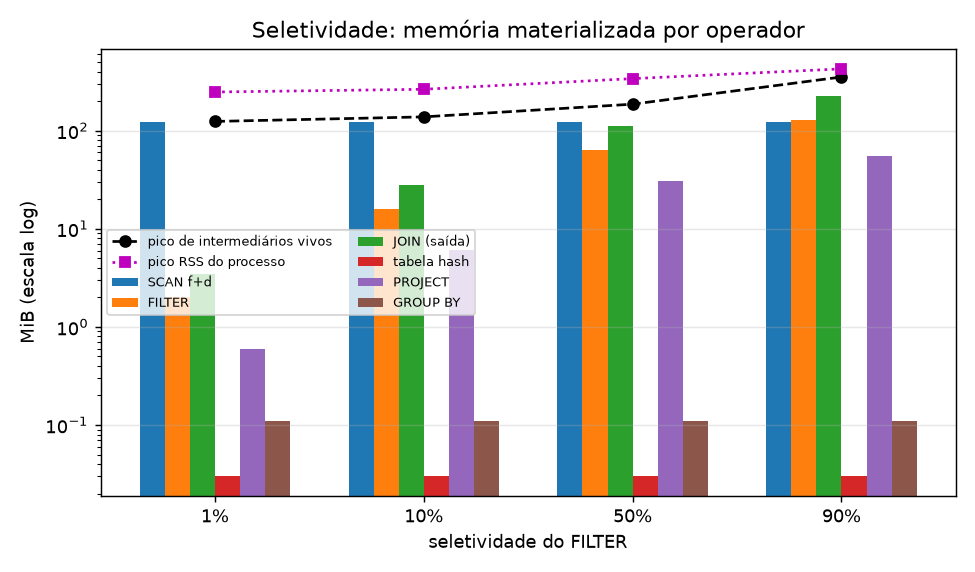
\includegraphics[width=0.82\linewidth]{seletividade_memoria.png}
\caption{Seletividade: memória reservada pelos intermediários.}
\label{fig:sel-mem}
\end{figure}

O FILTER decide quantas linhas chegam ao JOIN. De 1\% para 90\%, a entrada do JOIN cresce 92 vezes, e o tempo do JOIN acompanha: de 35 para 2\,530\,ms no Nested Loop e de 1,2 para 106,6\,ms no Hash Join. Já o tempo da consulta com Hash Join cresce só 4 vezes (80,6 para 324,9\,ms), porque o SCAN de \texttt{funcionarios} custa sempre cerca de 56\,ms e reserva sempre 122\,MiB, qualquer que seja o filtro. Com 1\%, SCAN e FILTER somam 97\% do tempo dos operadores. É o custo fixo da materialização: a cópia completa feita antes de o filtro descartar qualquer linha. A vantagem do Hash Join sobre o Nested Loop cresce com a seletividade: 1,6 vez com 1\%, 3,6 com 10\%, 7,1 com 50\% e 8,6 com 90\%.

\subsection{Tamanho da relação de BUILD}
Com 1 milhão de funcionários e \texttt{salary > 5000}, o número de departamentos variou de 100 a 100\,000. Como todo funcionário tem departamento, a saída do JOIN fica perto de 600 mil linhas em todos os casos, e só o tamanho do BUILD muda. O Nested Loop com 100\,000 departamentos ($6 \times 10^{10}$ comparações) foi executado por completo: 5 repetições, sem aquecimento, cerca de 4 minutos cada.

\begin{table}[H]
\centering
\footnotesize
\setlength{\tabcolsep}{3.5pt}
\begin{tabular}{@{}rlrrrrrrr@{}}
\toprule
Departamentos & Alg. & Linhas PROBE & Comparações & BUILD & PROBE & JOIN & Consulta & min--max \\
\midrule
100 & HJ & 599\,745 & 852\,072 & 0,004 & 70,1 & 70,1 & \textbf{252,0} & 246,0--275,9 \\
100 & NLJ & 599\,745 & 59\,974\,500 & 0,000 & 214,2 & 214,2 & \textbf{388,5} & 380,9--404,3 \\
\addlinespace[2pt]
1\,000 & HJ & 600\,178 & 879\,899 & 0,026 & 71,2 & 71,2 & \textbf{250,8} & 246,9--282,8 \\
1\,000 & NLJ & 600\,178 & 600\,178\,000 & 0,000 & 1\,809,1 & 1\,809,1 & \textbf{1\,998,0} & 1\,968,1--2\,088,9 \\
\addlinespace[2pt]
10\,000 & HJ & 599\,676 & 1\,154\,395 & 0,216 & 112,1 & 112,3 & \textbf{315,2} & 293,3--420,0 \\
10\,000 & NLJ & 599\,676 & 5\,996\,760\,000 & 0,000 & 16\,565,4 & 16\,565,4 & \textbf{16\,825,0} & 16\,050,3--18\,433,4 \\
\addlinespace[2pt]
100\,000 & HJ & 599\,556 & 1\,273\,291 & 2,896 & 135,5 & 138,4 & \textbf{387,2} & 378,6--388,3 \\
100\,000 & NLJ & 599\,556 & 59\,955\,600\,000 & 0,000 & 248\,502,4 & 248\,502,4 & \textbf{249\,065,3} & 235\,688,7--257\,660,8 \\
\bottomrule
\end{tabular}
\caption{Experimento de tamanho do BUILD: linhas, comparações e tempos (ms, mediana de 5 repetições).}
\label{tab:build-tempo}
\end{table}
\begin{table}[H]
\centering
\footnotesize
\setlength{\tabcolsep}{3.5pt}
\begin{tabular}{@{}rlrrrrrrrr@{}}
\toprule
Departamentos & Alg. & SCAN f & SCAN d & FILTER & JOIN & PROJECT & GROUP BY & Soma & JOIN/soma \\
\midrule
100 & HJ & 61,5 & 0,0 & 51,5 & 70,1 & 37,4 & 20,7 & 242,9 & 29\% \\
100 & NLJ & 56,8 & 0,0 & 49,8 & 214,2 & 37,2 & 20,4 & 380,3 & 56\% \\
\addlinespace[2pt]
1\,000 & HJ & 58,7 & 0,0 & 50,6 & 71,2 & 36,9 & 25,3 & 240,7 & 30\% \\
1\,000 & NLJ & 63,7 & 0,0 & 56,9 & 1\,809,1 & 40,5 & 26,6 & 1\,985,1 & 91\% \\
\addlinespace[2pt]
10\,000 & HJ & 61,0 & 0,5 & 56,0 & 112,3 & 38,9 & 31,0 & 296,9 & 38\% \\
10\,000 & NLJ & 73,5 & 0,6 & 61,9 & 16\,565,4 & 49,7 & 31,2 & 16\,809,1 & 99\% \\
\addlinespace[2pt]
100\,000 & HJ & 60,3 & 4,6 & 53,1 & 138,4 & 36,0 & 83,3 & 376,1 & 37\% \\
100\,000 & NLJ & 134,1 & 9,4 & 78,7 & 248\,502,4 & 114,4 & 88,1 & 248\,981,5 & 100\% \\
\bottomrule
\end{tabular}
\caption{Experimento de tamanho do BUILD: tempo de CPU por operador (ms, mediana).}
\label{tab:build-ops}
\end{table}
\begin{table}[H]
\centering
\footnotesize
\setlength{\tabcolsep}{3.5pt}
\begin{tabular}{@{}rrrrrrrrr@{}}
\toprule
Departamentos & SCAN f+d & FILTER & JOIN (saída) & Hash (KiB) & PROJECT & Total & Pico interm. & Pico RSS \\
\midrule
100 & 122,1 & 128,0 & 224,0 & 3,1 & 36,6 & 510,7 & 352,0 & 325,2 \\
1\,000 & 122,2 & 128,0 & 224,0 & 31,3 & 36,6 & 510,9 & 352,1 & 325,5 \\
10\,000 & 123,0 & 128,0 & 224,0 & 312,5 & 36,6 & 513,6 & 353,2 & 328,1 \\
100\,000 & 131,2 & 128,0 & 224,0 & 3\,125,0 & 36,6 & 536,9 & 364,2 & 353,4 \\
\bottomrule
\end{tabular}
\caption{Experimento de tamanho do BUILD: memória com Hash Join (MiB, salvo indicação). ``Total'' é a soma reservada por todos os intermediários.}
\label{tab:build-mem}
\end{table}
\begin{figure}[H]
\centering
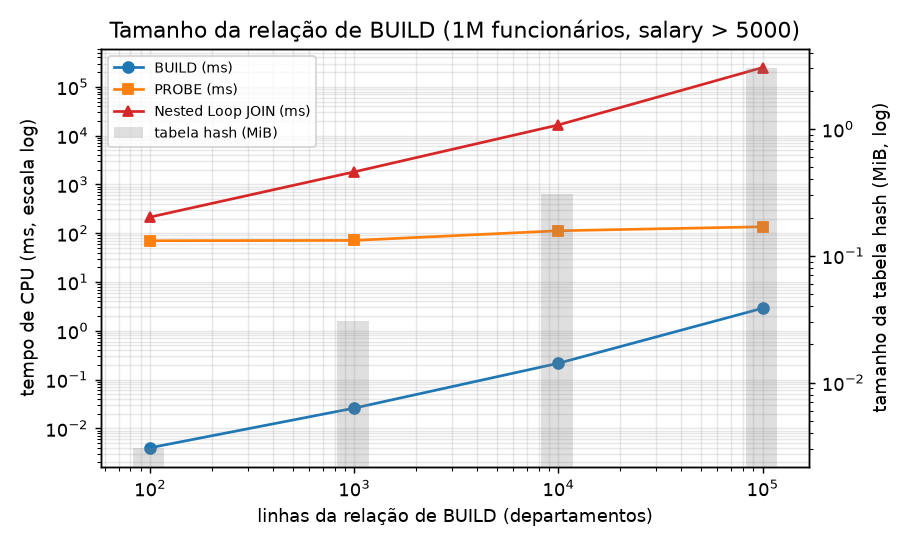
\includegraphics[width=0.82\linewidth]{build_tamanho.png}
\caption{Tamanho do BUILD: tempo de BUILD e PROBE e tamanho da tabela hash.}
\label{fig:build-tam}
\end{figure}

\begin{figure}[H]
\centering
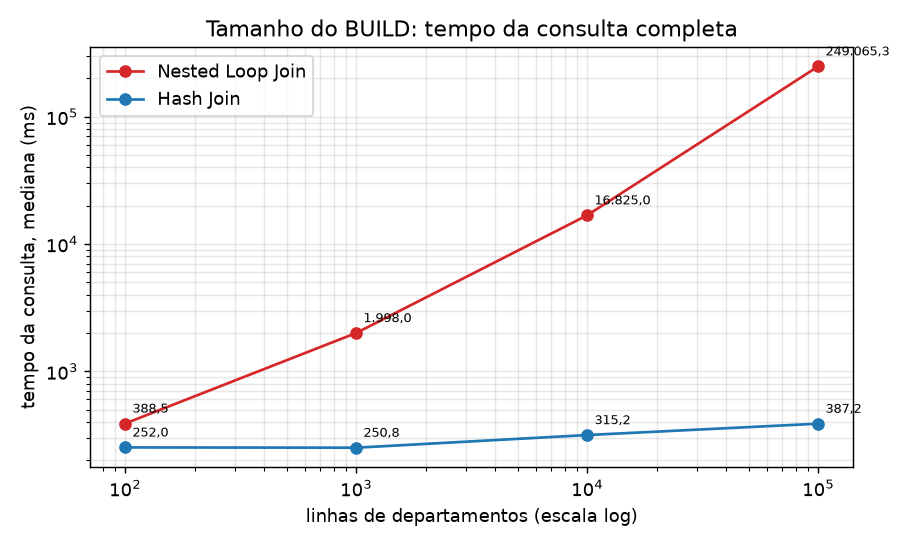
\includegraphics[width=0.82\linewidth]{build_tempo.png}
\caption{Tamanho do BUILD: tempo da consulta (mediana).}
\label{fig:build-tempo}
\end{figure}

O BUILD é barato e cresce de forma linear: 0,004\,ms com 100 linhas e 2,9\,ms com 100 mil, com a tabela hash indo de 3,1\,KiB para 3,1\,MiB. O PROBE quase dobra (de 70 para 135\,ms). Com 100 mil chaves, a tabela hash (3,1\,MiB) e as 100 mil linhas de \texttt{departamentos} (9,2\,MiB) já não cabem no cache L2 de 2\,MiB, e cada linha de PROBE faz mais acessos aleatórios. O número de comparações por linha de PROBE também sobe de 1,42 para 2,12, um pouco acima do 1,5 esperado para carga 0,5, o que indica que a função de hash espalha pior as chaves maiores. No Nested Loop, o JOIN cresce na proporção de $|D|$: de 214\,ms com 100 para 248\,502\,ms (4,1 minutos) com 100 mil departamentos, e o custo por comparação sobe de cerca de 3 para 4,1\,ns quando a relação interna deixa de caber no cache. Com 100 departamentos, o Nested Loop deixa a consulta só 1,5 vez mais lenta que o Hash Join; com 100 mil, 643 vezes.

\subsection{Tamanho do batch e comparações obrigatórias}
O teste de tamanho de batch (seção 8.4 do enunciado) não se aplica ao modelo materializado, porque não há lotes entre operadores, e o enunciado o atribui ao responsável pelo modelo vetorizado. A Tabela~\ref{tab:comparacoes} resume a situação das comparações da seção 9 do enunciado.

\begin{table}[H]
\centering
\small
\begin{tabular}{@{}p{7.4cm}p{9.0cm}@{}}
\toprule
Comparação & Situação \\
\midrule
Nested Loop $\times$ Hash Join & Medida (cardinalidade, seletividade e BUILD) \\
Materialização $\times$ Pipeline $\times$ Vetorizado & Não medida aqui: depende das implementações de JOIN dos Grupos B e C \\
Cardinalidades, seletividades e tamanhos de BUILD & Medidas \\
Tamanhos de batch & Não se aplica ao Grupo A \\
Memória, tempo total, tempo por operador, dados intermediários & Medidos (tabelas de tempo, de operadores e de memória) \\
\bottomrule
\end{tabular}
\caption{Comparações exigidas pelo enunciado.}
\label{tab:comparacoes}
\end{table}

Para que a comparação entre modelos seja justa, os três grupos precisam usar os mesmos datasets e a mesma consulta. O gerador e a semente desta etapa ficam no repositório para isso.

\section{Resposta à questão da etapa}\label{sec:questao}
\begin{quote}
\emph{Como o modelo de execução e o algoritmo de JOIN influenciam o custo de uma consulta composta por scan, filtro, join, projeção e agregação?}
\end{quote}

Nos experimentos do modelo materializado, o algoritmo de JOIN decide a ordem de grandeza do custo, e o modelo de execução decide o custo que sobra e, sobretudo, a memória.

\textbf{1. O algoritmo de JOIN define a complexidade.} O Nested Loop compara cada linha externa com todas as internas, então o custo é proporcional a $|F'| \times |D|$. O Hash Join paga $|D|$ para construir a tabela e cerca de 1,5 comparação por linha de PROBE. Com 1 milhão de funcionários e 1\,000 departamentos, foram 600 milhões de comparações contra 880 mil (682 vezes menos), e o JOIN caiu de 1\,645,6 para 71,6\,ms (23 vezes). O ganho em tempo é menor que o ganho em comparações porque cada passo do Hash Join custa mais (cálculo do hash, acesso aleatório à cadeia) e porque os dois algoritmos pagam a mesma materialização da saída (224\,MiB reservados). O tamanho da relação interna é o fator decisivo: com 100 departamentos, o Nested Loop deixa a consulta só 1,5 vez mais lenta; com 100 mil, 643 vezes (249\,s contra 0,39\,s). O Hash Join quase não sente essa variação (de 252 para 387\,ms), porque o BUILD custa no máximo 2,9\,ms.

\textbf{2. Filtrar antes do JOIN reduz o custo do JOIN na mesma proporção.} De 90\% para 1\% de seletividade, o JOIN do Nested Loop cai de 2\,530 para 35\,ms (72 vezes) e o do Hash Join de 106,6 para 1,2\,ms. Quanto mais caro o JOIN por linha, mais o filtro compensa; por isso a vantagem do Hash Join cai de 8,6 vezes (90\%) para 1,6 vez (1\%).

\textbf{3. Com Hash Join, o que sobra é o custo do modelo materializado.} Quando o JOIN é eficiente, ele responde por só 28 a 38\% do tempo. O resto é SCAN, FILTER, PROJECT e GROUP BY, e todos gravam a saída inteira. Só o SCAN de \texttt{funcionarios} (cópia completa) e o PROJECT (outra cópia) somam 36\% do tempo com 10 milhões de linhas (943 de 2\,611\,ms). Com seletividade de 1\%, SCAN e FILTER são 97\% do tempo, porque a tabela inteira é copiada antes de o filtro descartar 99\% dela. Na memória, a consulta de 10 milhões reserva 4,3\,GiB de intermediários (SCAN 1,19\,GiB, FILTER 1\,GiB, JOIN 1,75\,GiB, PROJECT 366\,MiB) para devolver 1\,000 linhas. O pico de intermediários vivos chega a 2,75\,GiB, e o pico de RSS do processo a 3,2\,GiB. A tabela hash ocupa só 31\,KiB desse total: no modelo materializado, quem consome memória são as tabelas intermediárias, e não a estrutura do JOIN.

\textbf{4. O modelo muda o papel de BUILD e PROBE.} No modelo materializado, o BUILD não espera mais do que esperaria de qualquer forma, porque a relação de \texttt{departamentos} já está completa. O PROBE, porém, também recebe a entrada inteira e materializa toda a saída, que é o maior intermediário da consulta. Nos modelos pipeline e vetorizado, que não foram medidos aqui, o esperado pelo funcionamento dos operadores é que o BUILD continue sendo um ponto de bloqueio (a tabela hash precisa estar completa antes do primeiro PROBE), mas que o PROBE, o PROJECT e o GROUP BY passem a consumir as linhas à medida que elas chegam. Assim, os gigabytes de tabelas intermediárias dariam lugar à tabela hash e ao estado dos grupos (cerca de 145\,KiB com 1\,000 departamentos), mais um lote por operador no vetorizado. Em troca, haveria custo de chamada por tupla (pipeline) ou por lote (vetorizado). Quanto isso custa de fato só pode ser respondido com as medições dos Grupos B e C nos mesmos datasets.

\textbf{Conclusão.} O custo da consulta é aproximadamente o custo do JOIN mais um custo proporcional ao volume de dados copiado entre os operadores. O algoritmo de JOIN define o primeiro termo: o Nested Loop o torna quadrático e dominante (90 a 100\% do tempo quando $|D| \geq 1\,000$), e o Hash Join o torna linear e secundário. O modelo de execução define o segundo: no modelo materializado, cada operador copia a sua saída inteira, o que, com Hash Join, responde pela maior parte do tempo e por toda a memória que cresce com os dados. Filtros seletivos antes do JOIN reduzem os dois termos, exceto a cópia do SCAN, que a materialização paga sempre.

\section{Dificuldades encontradas}\label{sec:dificuldades}
\begin{itemize}
    \item \textbf{Memória da linha fixa.} A \texttt{Row} de 2176 bytes da etapa 2 inviabilizava as cardinalidades pedidas: 10 milhões de linhas ocupariam cerca de 20\,GiB por tabela. A solução foi a tabela compacta (Seção~\ref{sec:compacta}), que exigiu trocar todos os acessos \texttt{rows[i].values[j]} por funções de acesso.
    \item \textbf{GROUP BY linear.} A busca linear pelos grupos funcionava nos testes, mas tornaria o experimento com 100 mil departamentos inviável. Foi trocada por um índice hash, mantendo a ordem dos grupos que os testes já verificavam.
    \item \textbf{Custo do Nested Loop nos experimentos.} Com 100 mil departamentos, cada execução leva cerca de 4 minutos. Mesmo assim, as 5 repetições foram feitas, só sem a rodada de aquecimento.
    \item \textbf{Medição.} \texttt{clock()} mede tempo de CPU por operador, e o tempo da consulta inteira precisou de relógio de parede (\texttt{timespec\_get}). A memória reservada e a física são diferentes, por isso ambas são reportadas. A máquina compartilhada introduz ruído de até cerca de 10\% entre processos.
    \item \textbf{Datasets grandes no GitHub.} Os arquivos de 5 e 10 milhões passam dos limites de um repositório comum, por isso ficam fora do Git e são gerados de forma determinística.
\end{itemize}

\section{Limitações atuais}\label{sec:limitacoes}
\begin{itemize}
    \item Só o modelo materializado, sem comparação medida com pipeline e vetorizado.
    \item Só INNER JOIN com uma condição de igualdade. Não há planner: o algoritmo é escolhido pelo chamador, e só o lado de BUILD é automático.
    \item Não há parser SQL; as consultas são montadas no código.
    \item CSV simples: sem aspas, sem \texttt{NULL} e sem validação do cabeçalho; strings de até 23 caracteres; no máximo 16 colunas por tabela.
    \item Não há verificação de memória disponível antes de materializar: uma entrada grande demais termina em falha de alocação (tratada, com liberação).
    \item Tempos de operador em tempo de CPU; consulta inteira em tempo de parede.
    \item O FILTER aceita um único predicado.
\end{itemize}

\section{Possíveis otimizações futuras}\label{sec:otimizacoes}
As otimizações a seguir partem de medições desta etapa.
\begin{enumerate}
    \item \textbf{SCAN sem cópia, ou fundido com o FILTER.} O SCAN custa de 22 a 23\% do tempo e 1,19\,GiB com 10 milhões; com seletividade de 1\%, SCAN e FILTER são 97\% do tempo.
    \item \textbf{Projeção antecipada.} A saída do JOIN tem 7 colunas (224 bytes por linha) e é o maior intermediário, mas só 2 colunas são usadas depois. O JOIN poderia gravar só \texttt{d.name} e \texttt{f.salary}.
    \item \textbf{Agregação no próprio PROBE.} Fundir o GROUP BY ao JOIN eliminaria a saída do JOIN e a do PROJECT (2,1\,GiB com 10 milhões).
    \item \textbf{Melhor função de hash ou endereçamento aberto.} Com 100 mil chaves foram 2,12 comparações por linha de PROBE, contra 1,5 esperado.
    \item \textbf{Estimar a capacidade da saída do FILTER e do JOIN.} A capacidade dobra e chega a reservar quase o dobro do usado: o FILTER de 10 milhões reservou 1\,GiB para 732\,MiB de linhas.
    \item \textbf{Strings fora da linha.} O \texttt{Value} de 32 bytes existe por causa da string de 24 bytes, e as colunas numéricas pagam esse tamanho.
    \item \textbf{Armazenamento colunar.} PROJECT e GROUP BY leem 2 de 7 colunas.
    \item \textbf{Planner simples.} Escolher Nested Loop só quando $|R| \times |S|$ for pequeno.
    \item \textbf{Hash Join particionado (grace).} Para quando a relação de BUILD não couber na memória.
\end{enumerate}

\section{Material de extensão}\label{sec:extensao}
O material de extensão desta etapa é um vídeo curto, de 3 a 5 minutos, sobre o tema ``Nested Loop Join versus Hash Join e a fase de BUILD''. O vídeo mostra, no código, os dois laços do Nested Loop e as fases de BUILD e PROBE do Hash Join, e faz duas demonstrações no terminal. A primeira executa a consulta completa com 1 milhão de funcionários e 1\,000 departamentos e compara as métricas dos dois JOINs:
\par\medskip\noindent\begin{minipage}{\linewidth}
\begin{lstlisting}
python3 bench/generate_data.py --employees 1000000 --departments 1000 \
    --employee-file /tmp/demo/funcionarios_1m.csv \
    --department-file /tmp/demo/departamentos_1k.csv
./miniquery /tmp/demo/funcionarios_1m.csv /tmp/demo/departamentos_1k.csv
\end{lstlisting}
\end{minipage}\par\medskip
Nessa execução, o Nested Loop faz 600\,178\,000 comparações e o Hash Join 879\,899, com uma tabela hash de 32\,008 bytes. A segunda demonstração varia só o lado de BUILD (100 e 100\,000 departamentos) com \texttt{miniquery\_bench}, para mostrar que o BUILD continua na casa dos milissegundos enquanto a tabela hash cresce de 3\,208 para 3\,200\,008 bytes.

\section{Como reproduzir}
\par\medskip\noindent\begin{minipage}{\linewidth}
\begin{lstlisting}
make && ./miniquery          # consulta no dataset versionado
make test && make sanitize && make valgrind
make experiments             # gera os datasets (~440 MB) e mede tudo
python3 bench/summarize.py   # medianas, tabelas e graficos
\end{lstlisting}
\end{minipage}\par\medskip
O Nested Loop com 100 mil departamentos leva cerca de 21 minutos no total. Para rodar só uma parte: \texttt{python3 bench/run\_experiments.py --only seletividade}.

\section{Conclusão}
A etapa 3 acrescenta ao motor materializado do Grupo A o suporte a duas tabelas, o Nested Loop Join, o Hash Join com BUILD na menor relação e PROBE explícitos, o GROUP BY por hash e a instrumentação pedida pelo enunciado. Os dois algoritmos devolvem os mesmos resultados em todos os testes e experimentos. Com Hash Join, a consulta sobre 10 milhões de funcionários levou 2,7\,s, contra 19,9\,s com Nested Loop, e a diferença chega a 643 vezes quando a relação de BUILD tem 100 mil linhas. Com o JOIN eficiente, o custo restante e a memória vêm da materialização dos intermediários, e não da tabela hash. A validação com Valgrind terminou sem vazamentos e sem erros em todos os programas.

{\small
\begin{thebibliography}{9}
\bibitem{graefe}
G. Graefe.
\newblock Query evaluation techniques for large databases.
\newblock \emph{ACM Computing Surveys}, 25(2):73--169, 1993.

\bibitem{garcia}
H. Garcia-Molina, J. D. Ullman e J. Widom.
\newblock \emph{Database Systems: The Complete Book}.
\newblock 2.\ ed. Pearson Prentice Hall, 2008.

\bibitem{valgrind}
Valgrind Developers.
\newblock \emph{Valgrind User Manual -- Memcheck: a memory error detector}.
\newblock Disponível em: \url{https://valgrind.org/docs/manual/mc-manual.html}.
\end{thebibliography}
}

\end{document}
